\begin{figure}[h]
	%\centering
	\hspace{-0.25\linewidth}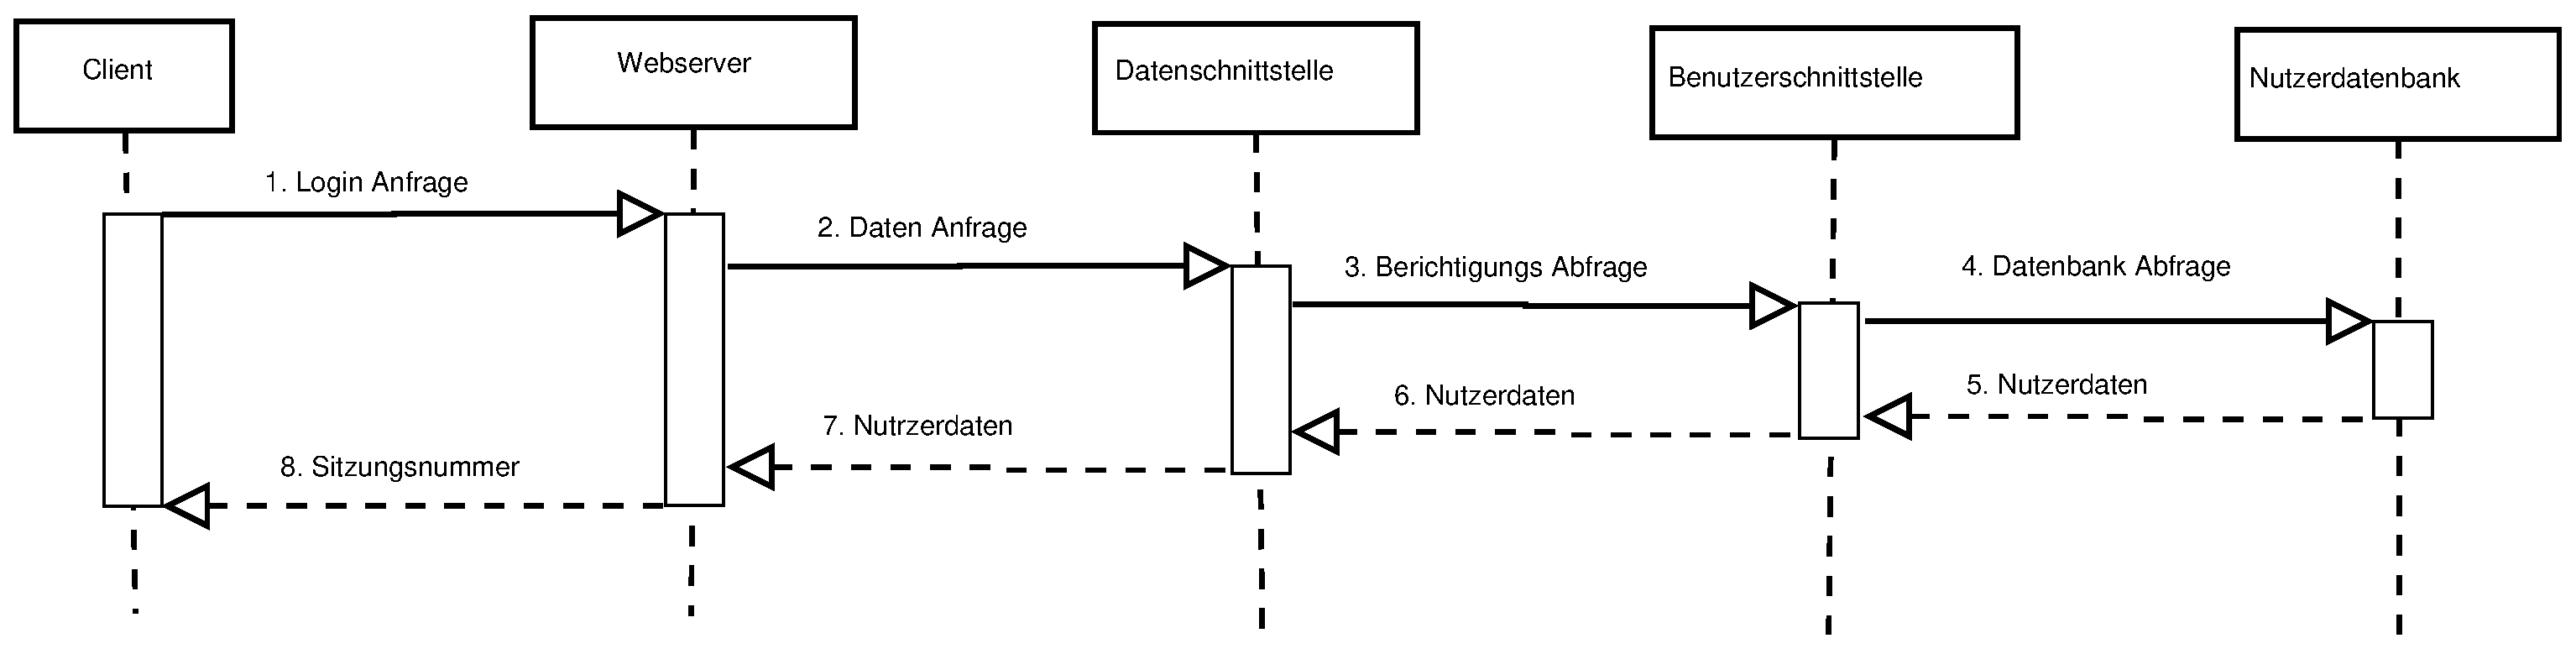
\includegraphics[width=1.5\linewidth]{Grafik/Diagramm/Szenarios/Login}
	\caption[]{Anmeldung eines Benutzers}
\end{figure}

\noindent Nachdem der Benutzer die Startseite aufgerufen hat, kann er sich über ein Formular auf der Seite anmelden. Nach dem Klick auf die entsprechende Schaltfläche wird eine Login Anfrage an den Webserver geschickt. Dieser beauftragt die Datenschnittstelle die erforderlichen Nutzerdaten abzufragen. Hierzu wird die Benutzerschnittstelle angesprochen, die prüft, ob es sich bei den Anmeldedaten um einen registrierten und zugangsberechtigten Nutzer handelt. Sollte dies der Fall sein, so werden die angeforderten Daten aus der Nutzerdatenbank ausgelesen und in der selben Hierarchie bis zum Webserver nach oben gereicht. Dort angelangt wird dem Nutzer eine Sitzungsnummer zugewiesen und ihm zu Zugang zu seinem Account gewährt. 